The data-driven algorithm described so far uses the forecast of features to obtain building power consumption predictions. 
In this section, we describe a control algorithm which utilizes the multi-variate output capability of our regression tree model to implement receding horizon control. This is also one of our primary contributions.

%Recall that the objective of learning a regression tree is to learn a model $f$ for predicting the response $\mathbb{Y}$ with the values of the predictor variables or features $\mathbb{X}^1, \dots, \mathbb{X}^n$; i.e. $Y=f(\mathbb{X}^1, \dots, \mathbb{X}^n)$.
%Given a forecast of the features $\hat{X}^1, \dots, \hat{X}^n$ we can predict the response $\hat{Y}$. 
%Now consider the case where a subset, $\mathbb{X}_c \subset \mathbb{X}$ of the set of features/variables $\mathbb{X}$'s are manipulated variables i.e. we can change their values in order to drive the response $\mathbb{Y}$ towards a certain value. 
%In the case of buildings, the set of  variables can be separated into disturbances (or non-manipulated) variables like outside air temperature, humidity, wind etc. while the controllable (or manipulated) variables would be the temperature and lighting set-points within the building.
%Our goal is to modify the regression trees and make them suitable for synthesizing the optimal values of the control variables in real-time.
In Sec.~\ref{sec:drsyn} an algorithm for model based control with regression trees (mbCRT) \cite{BehlJainMangharam2016,Behl201630} was presented. This algorithm utilizes a \emph{separation of variables} principle to allow for a control optimization in the leaves of the tree. 
Although mbCRT enables control with regression trees based models, it suffers from two significant limitations:
\begin{enumerate}
\item mbCRT is based on uni-variate output regression tree models and is unable to make multi-variate predictions. 
\item The mbCRT algorithm is a `one-step look-ahead' algorithm. It can only account for an unexpected disturbance only one time-step before it occurs, thus making it sub-par as compared to receding horizon control algorithms.
\end{enumerate}

\begin{figure}
\centering
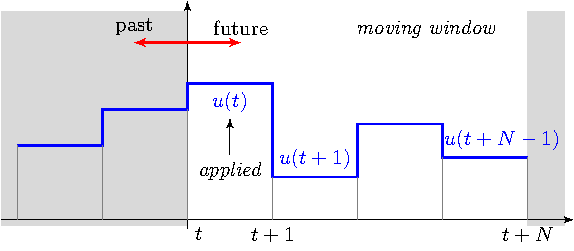
\includegraphics[scale=0.85]{Figures/receding_horizon.pdf}
\caption{Finite-horizon moving window of MPC: at time $t$, the MPC optimization problem is solved for a finite length window of $N$ steps and the first control input $u(t)$ is applied; the window then recedes one step forward and the process is repeated at time $t+1$.}
\captionsetup{justification=centering}
\label{F:MPC-illust}
\end{figure} 

%In mbCRT, given building data $(\mathbb{X},\mathbb{Y})$ in the form of \eqref{E:dataset}, we can separate the controllable $\mathbb{X}_c$ (or manipulated variables) and uncontrollable variables $\mathbb{X}_d$ (or non-manipulated variables or disturbances) in the features such that $\mathbb{X}_c \cup \mathbb{X}_d \equiv \mathbb{X}$. 
%This is called separation of variables.
%Applying this separation of variables, the regression tree is built only on the non-manipulated variables or disturbances $(\mathbb{X}_d,\mathbb{Y})$.  
%We obtain a model in the following form:
%\begin{gather}
%\mathbb{Y} = \mathit{f} \left( \mathbb{X}^1_d,\dots,\mathbb{X}^n_d \right).
%\label{E:train_model_single}
%\end{gather}
%In the leaf $R_i$ of the tree, we fit a parametric model (linear regression) which is a function only of the controllable/manipulated variables:
%\begin{gather}
%\mathbb{Y}_{R_i} = \beta_{0,i} + \beta^T_i \mathbb{X}_c.
%\end{gather}
%In this manner, we train a regression tree using only $\mathbb{X}_d$, and then in each leaf we train a linear model which is a function only of $\mathbb{X}_d$. 
%To solve the control problem when only $\mathbb{X}_d$ is known, we navigate to an appropriate leaf $R_i$ and determine $\mathbb{X}_c$ from the following optimization problem:
%\begin{align}
%\begin{aligned}
%\text{minimize } \ \ \ & \ \ \ \ \ \ \mathit{g} \left( \mathbb{Y}_{R_i}, \mathbb{X}_c  \right) \\ \text{subject to } \ \ \ & \mathbb{Y}_{R_i} = \beta_{0,i} + \beta^T_i \mathbb{X}_c, \\ \ \ \ & \ \ \ \ \ \ \mathbb{X}_c \in \mathbb{X}_{\mathrm{des}},
%  \end{aligned}
%  \label{E:opt_single}
%\end{align}
%where $g$ is some function of the response variable and/or control variables we wish to minimize.

The finite receding horizon control approach involves optimizing a cost function subject to the dynamics of the system and the constraints, over a finite horizon of time. 
After an optimal sequence of control inputs are computed, the first input is applied, then at the next step the optimization is solved again as shown in Fig. \ref{F:MPC-illust}. 

In the following section, we extend the mbCRT algorithm such that we can implement receding horizon control and address the limitations in mbCRT.  
This algorithm is called data predictive control with regression trees (DPCRT).

\begin{algorithm}[t]
\caption{DPCRT: Data Predictive Control with Regression Trees}
\label{A:DPC}
\begin{algorithmic}[]
\State \textsc{Design Time}
\Procedure{Model Training using Separation of Variables}{}
\State Set $\mathbb{X}_c$ $\gets$ manipulated features
\State Set $\mathbb{X}_d$ $\gets$ non-manipulated features
\State Build predictive tree(s) $\mathfrak{T}$(s) with $(\mathbb{Y},\mathbb{X}_d)$ using \eqref{E:regtree_multi}
\ForAll{regions $R_i$ at the leaves of $\mathfrak{T}$}
\State Choose a function $h$ for the problem
\State Fit linear model $\mathit{h} \left( \mathbb{Y}_{R_i}^1, \dots, \mathbb{Y}_{R_i}^p \right) = \beta_{0,i} + \beta^T_i \mathbb{X}_c$
\EndFor
\EndProcedure
\State \textsc{Run Time}
\Procedure{Predictive Control}{}
\While{$t< t_{\mathrm{stop}}$}
\State Determine the leaf and region $R_{i}(t)$ using $\mathbb{X}_d(t)$
\State Obtain the linear model at $R_{i}(t)$
\State Choose a cost function $g$ for the problem
\State Solve optimization in \eqref{E:opt_multi} or \eqref{E:opt_multi2} to determine optimal control action $\left[\mathbb{X}^*_c(t),\dots,\mathbb{X}^*_c(t+p)\right]^T $
\State Apply the first input $\mathbb{X}^*_c(t)$
\EndWhile
\EndProcedure
\end{algorithmic}
\end{algorithm}

\begin{figure*}[b!]
\centering
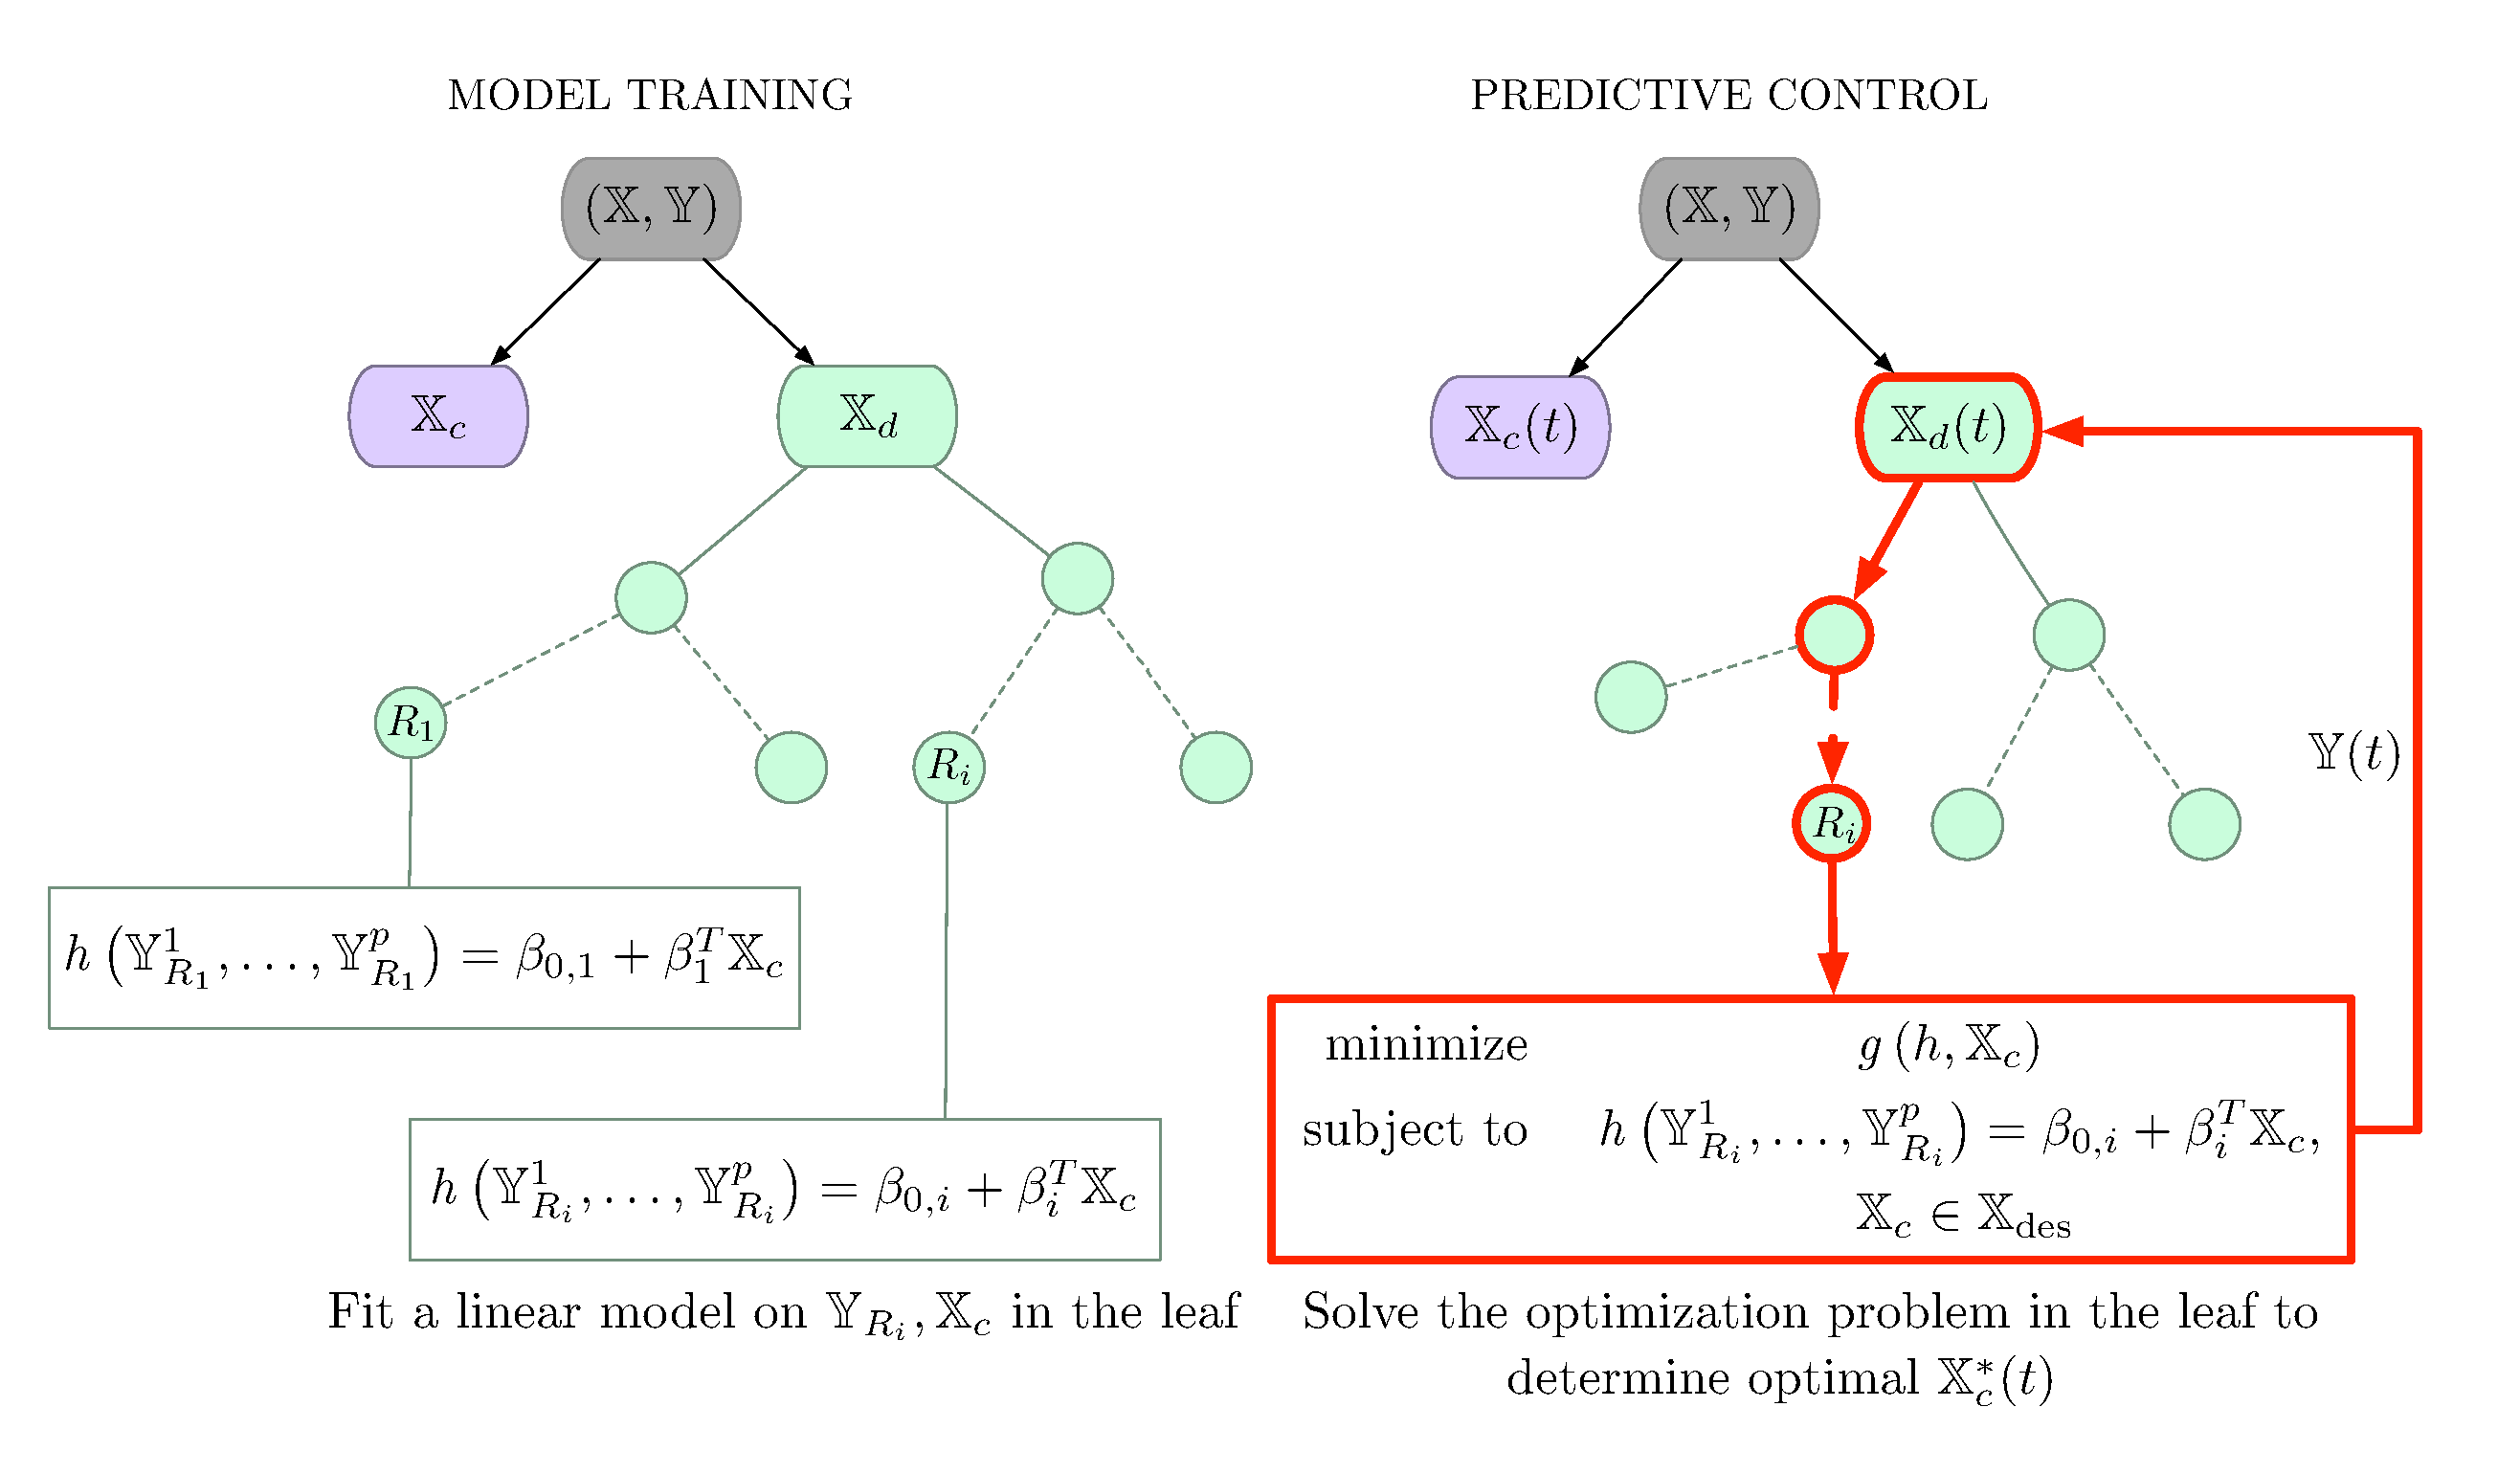
\includegraphics[width=0.95\linewidth]{Figures/DPC_tree2.eps}
\caption{Data Predictive Control with Regression Trees with Model Training Process (L) and Receding Horizon Control (R). During control step, the optimal control action $\left[\mathbb{X}^*_c(t),\dots,\mathbb{X}^*_c(t+p)\right]^T $ is determined. The first input $\mathbb{X}^*_c(t)$ is applied to the system. The resulting output $\mathbb{Y}(t)$ which is a feature for the next time step is fed back to determine to determine $R_{i}(t+1)$.}
\captionsetup{justification=centering}
\label{F:DPC_schematic}
\end{figure*}

\subsection{Data predictive control with Regression Trees}
\label{SS:control_algo}

The central idea behind DPCRT is to build a tree model which can also predict future states of the system. Thus, while training a regression tree with multiple response variables, we still use separation of variables as in mbCRT, the difference lies in the number of output variables in each leaf. Therefore, we generate a regression tree of the form
\begin{gather}
\begin{pmatrix}
\mathbb{Y}^1 \\ \vdots \\ \mathbb{Y}^p
\end{pmatrix}
 = \mathit{f} \left( \mathbb{X}^1_d,\dots,\mathbb{X}^n_d \right).
\label{E:train_model_multi}
\end{gather}
In each leaf of the tree, we now fit a linear model on a function $h : \mathbb{R}^p \to \mathbb{R}$ of all the response variables such that
\begin{gather}
\mathit{h} \left( \mathbb{Y}_{R_i}^1, \dots, \mathbb{Y}_{R_i}^p \right) = \beta_{0,i} + \beta^T_i \mathbb{X}_c.
\label{E:linear_leaf}
\end{gather}
A simple example of $h$ is an affine function which we will use for our case study in Sec. \ref{SS:case_dpc}. Once the model is trained, we solve the following optimization problem:
\begin{align}
\begin{aligned}
\text{minimize } \ \ \ & \ \ \ \ \ \ \ \ \ \ \ \ \ \ \ \mathit{g} \left( h, \mathbb{X}_c  \right) \\ \text{subject to } \ \ \ & \mathit{h} \left( \mathbb{Y}_{R_i}^1, \dots, \mathbb{Y}_{R_i}^p \right) = \beta_{0,i} + \beta^T_i \mathbb{X}_c, \\ \ \ \ & \ \ \ \ \ \ \ \ \ \ \ \ \ \ \ \mathbb{X}_c \in \mathbb{X}_{\mathrm{des}}.
  \end{aligned}
  \label{E:opt_multi}
\end{align}

We solve this optimization in the same manner as finite receding horizon control, and $\mathbb{X}_c$ includes all the control variables for the chosen horizon, i.e. $\mathbb{X}_c := \left[\mathbb{X}_c(t), \dots, \mathbb{X}_c(t+p)\right]^T$. We choose the first optimal control input $\mathbb{X}_c^*(t)$ and proceed to the next time step.

If the number of control variables is large, the optimization problem \eqref{E:opt_multi} may require many data points in the leaves or in other words a large $minLeaf$ which can affect the accuracy of the regression tree. 
Therefore, we also introduce a variant of this algorithm which will ease the selection of a lower $minLeaf$:
\begin{align}
\begin{aligned}
\text{minimize } \ \ \ & \ \ \ \ \ \ \ \ \ \mathit{g} \left( h^1, \dots, h^{\mathrm{nc}}, \mathbb{X}_c  \right) \\ \text{subject to } \ \ \ & \mathit{h}^1 \left( \mathbb{Y}_{R_i}^1, \dots, \mathbb{Y}_{R_i}^p \right) = \beta_{0,i} + \beta^T_i \mathbb{X}_c^1, \\ \ \ \ & \ \ \ \ \ \ \ \ \ \ \ \ \ \ \ \ \ \ \vdots \\ \ \ \ & \mathit{h}^{\mathrm{nc}} \left( \mathbb{Y}_{R_i}^1, \dots, \mathbb{Y}_{R_i}^p \right) = \gamma_{0,i} + \gamma^T_i \mathbb{X}_c^{\mathrm{nc}}, \\ \ \ \ & \ \ \ \ \ \ \ \ \ \ \ \ \ \ \ \mathbb{X}_c \in \mathbb{X}_{\mathrm{des}}.
  \end{aligned}
  \label{E:opt_multi2}
\end{align}


Here, $h^j$ is a linear model which depends only in the control variable $\mathbb{X}_c^j$. Note that $\mathbb{X}_c^j$ can still be a vector when horizon length is greater than 1. With suitable choice of $g$ and $h$, the problems \eqref{E:opt_multi} and \eqref{E:opt_multi2} can be formed as convex optimization problems. 

Our algorithm for DPC with regression trees in summarized in Algo. \ref{A:DPC} and a schematic is shown in Fig. \ref{F:DPC_schematic}. During training process, the tree is trained only on uncontrollable variables with linear models in the leaves which are a function only of controllable variables. During the control step, at time $t$, the uncontrollable features $\mathbb{X}_d(t)$ are known and thus the leaf $R_{i}(t)$ is known. The optimization problem in $R_i(t)$ is solved to determine the control action $\left[\mathbb{X}^*_c(t),\dots,\mathbb{X}^*_c(t+p)\right]^T $. The first input $\mathbb{X}^*_c(t)$ is applied to the system. The resulting output $\mathbb{Y}(t)$ which is a feature for the next time step is fed back to determine to determine $R_{i}(t+1)$.
In the context of a building model, we show the efficacy of DPCRT in Sec. \ref{SS:DPC_model_validation}.

\subsection{Model Validation: DPCRT}
\label{SS:DPC_model_validation}

\begin{figure}
\subfigure[Building power consumption at time $T$ predicted at time $T$ is denoted by $\mathcal{P}_{T}$, predicted 10 steps ahead at time $T-10$ is denoted by $\mathcal{P}_{T+10}$, and predicted 20 steps ahead at time $T-20$ is denoted by $\mathcal{P}_{T+20}$]{
\centering
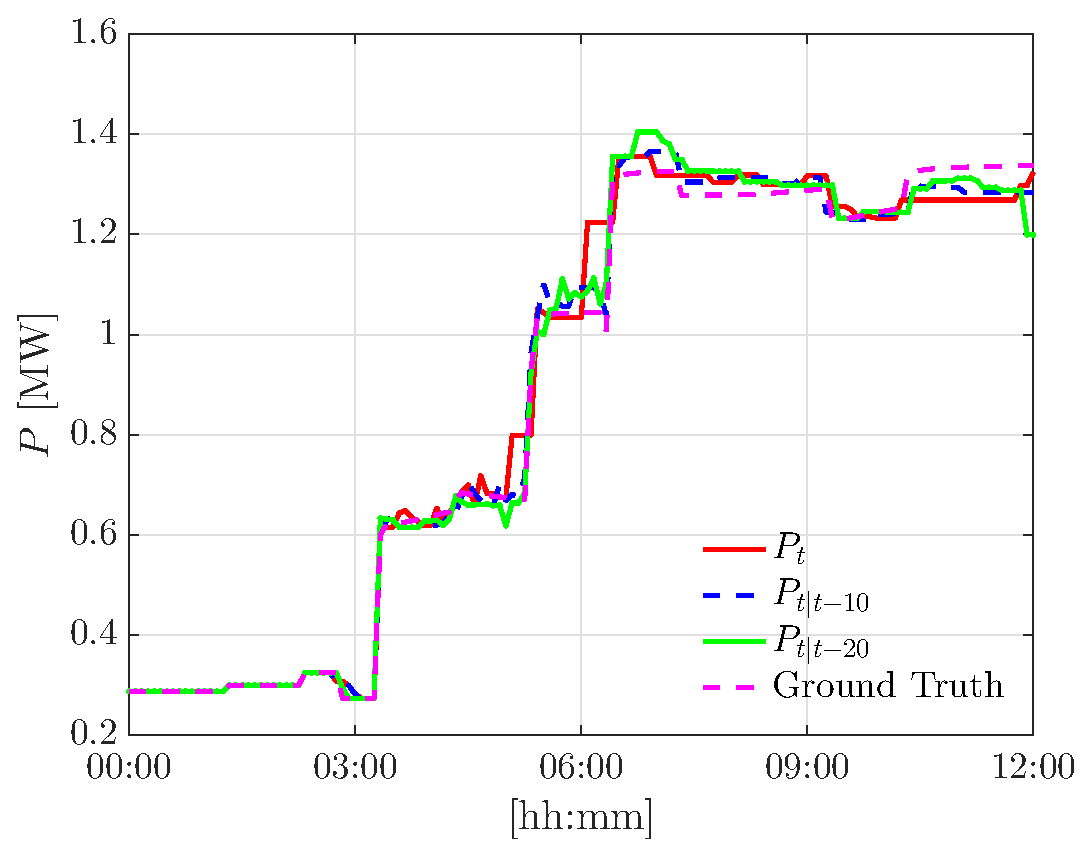
\includegraphics[width=18pc]{Figures/perf_test.eps}
\label{F:perf_test}
}
\subfigure[A comparison of power consumption of the building for two different regression trees. $\mathcal{T}_1$ is trained on all the features while $\mathcal{T}_2$ is trained only on non-manipulated features using separation of variables.]{
\centering
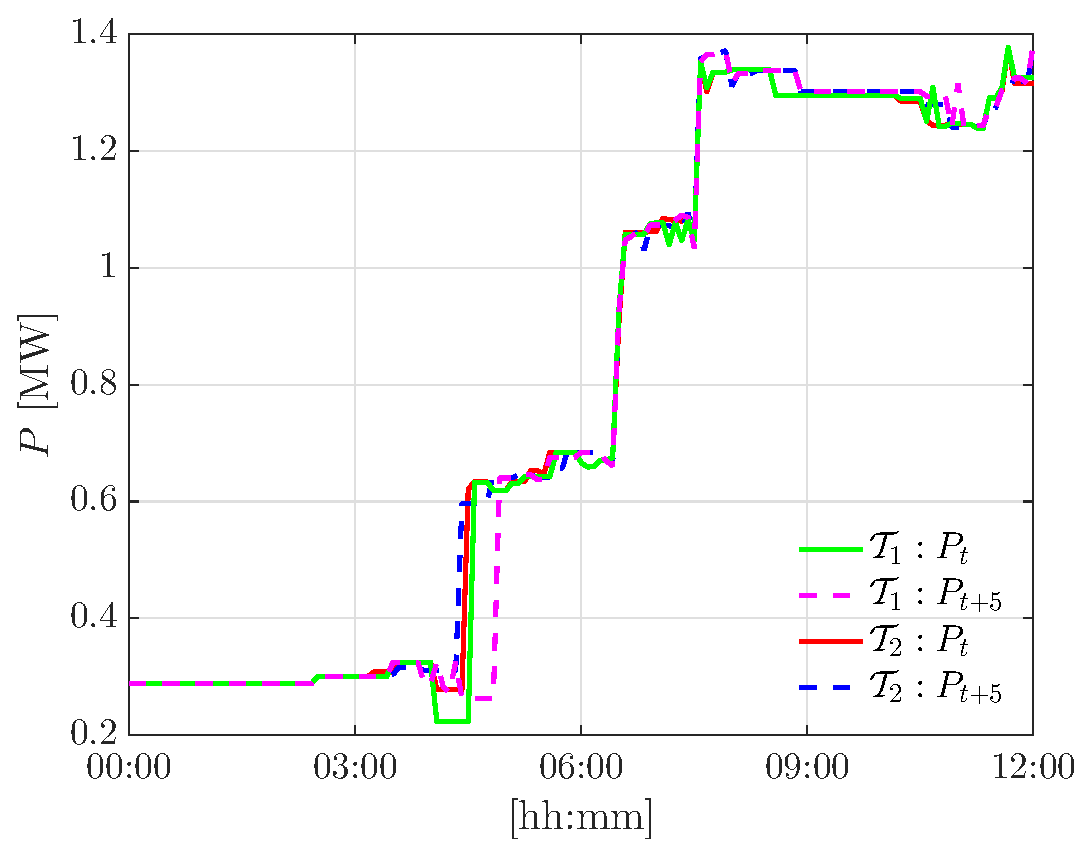
\includegraphics[width=18pc]{Figures/separation_vars.eps}
\label{F:separation_vars}
}
\subfigure[Model validation for linear regression at the leaves of the tree. The predicted and the actual power consumption are very close.]{
\label{F:linear_approx2}
\centering
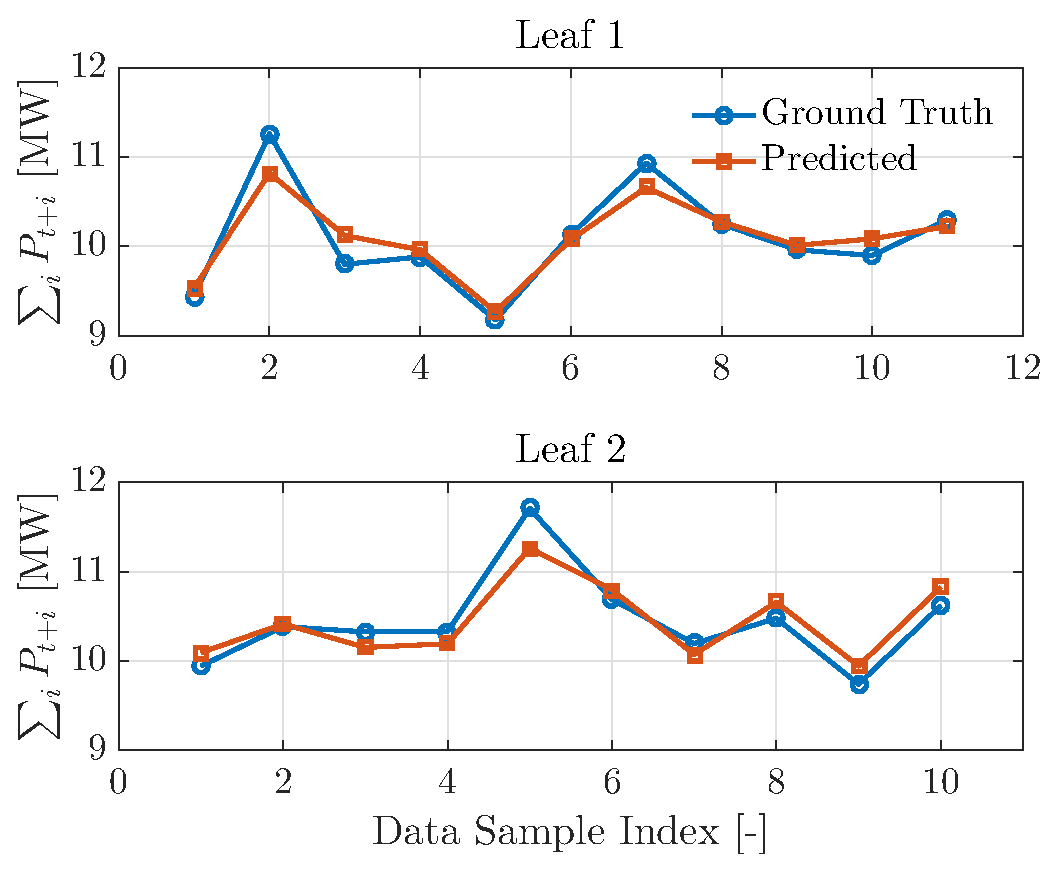
\includegraphics[width=18pc]{Figures/error_leaf2_1.eps}
}
\subfigure[The tree has 703 leaves. For each leaf, a maximum and a minimum error in prediction of average power consumption over the control horizon $\mathcal{P}_{\mathrm{pred}}-\mathcal{P}_{\mathrm{act}}$ is calculated from the data points that end up in that leaf.]{
\centering
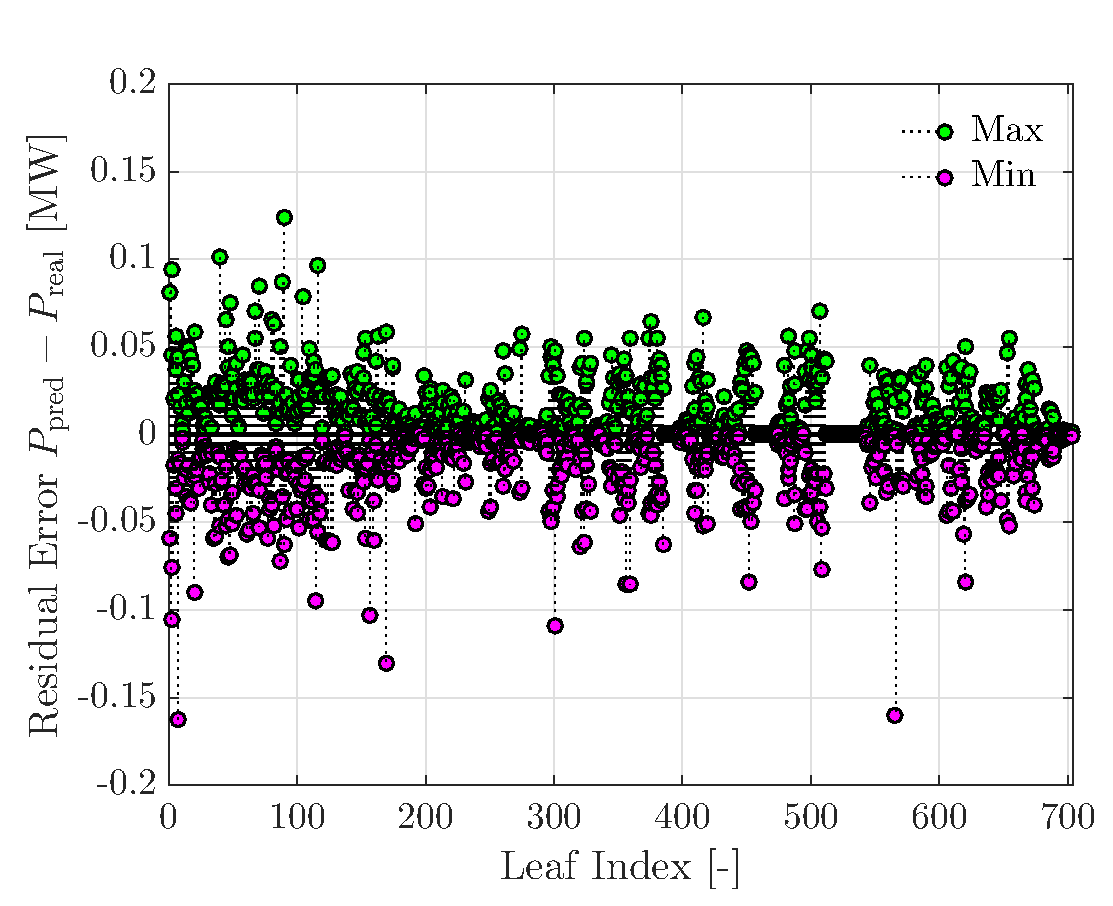
\includegraphics[width=18pc]{Figures/error_leaf.eps}
\captionsetup{justification=centering}
\label{F:linear_approx}
}
\caption{Model Validation of DPCRT.}
\captionsetup{justification=centering}
\end{figure}

The performance of DPCRT depends on two key assumptions: (a) first, is that the separation of variables doesn't introduce significant errors while training the tree, and (b) second, that the linear regression at the leaves is a valid assumption.
We verify the validity of these assumptions in terms of their effect on model accuracy.

\subsubsection{Separation of Variables}
We train two kinds of regression trees: (1) a tree $\mathcal{T}_1$ that has all the features as described earlier, and (2) a tree $\mathcal{T}_2$ that was learned from non-manipulated variables only with a linear model on the control/manipulated variables at the leaves.
%These 3 features are considered to be the control variables. 
%In other words, $\mathcal{T}_1$ is trained on all the features $\mathbb{X}$ while $\mathcal{T}_2$ is trained only on non-manipulated features $\mathbb{X}_d$. 
The predicted power consumption of the building at time $T$ and $T+5$ (see \eqref{E:building_model}), i.e. $\mathcal{P}_T$ and $\mathcal{P}_{T+5}$, respectively, for both trees is shown in Fig. \ref{F:separation_vars}. The normalized root mean square error (NRMSE) for these 2 outputs on the test dataset is shown in Tab. \ref{T:NMRSE_separation_vars}. We notice a small loss in model accuracy with $\mathcal{T}_2$ due to the separation of variables. 
This is the opportunity cost for integrating control synthesis with the tree, since otherwise the control features would have been a part of the splitting criteria rather than a linear model in the leaves of the tree.
%As seen in Fig. \ref{F:separation_vars} and Tab. \ref{T:NMRSE_separation_vars}, this error is not significant. 
In the case of $\mathcal{T}_2$ we exploit the tree structure to reach the right leaf, the actual output is determined by fitting a linear model which is a function of the controlled variables.

\begin{table}
  \centering
  \caption{NRMSE for regression trees with $(\mathcal{T}_1)$ and without $(\mathcal{T}_2)$ controllable features.}
    \begin{tabular}{c|c|c|c|c|c|c}
    \toprule
     & $\mathcal{P}_{T}$ &$\mathcal{P}_{T+1}$ &$\mathcal{P}_{T+2}$ &$\mathcal{P}_{T+3}$ &$\mathcal{P}_{T+4}$ & $\mathcal{P}_{T+5}$ \\
    \midrule
    $\mathcal{T}_1$     & 0.1037  &  0.1036 &   0.1116 &   0.1124 &   0.1140  &  0.1164  \\
    $\mathcal{T}_2$     & 0.1156  &  0.1182 &   0.1270 &   0.1268 &   0.1324  &  0.1308  \\
    \bottomrule
    \end{tabular}
  \label{T:NMRSE_separation_vars}
\end{table}

\subsubsection{Linear Approximation at Leaves}
For the tree $\mathcal{T}_2$, we fit a linear model on the sum of all outputs, i.e. the sum of power consumption over the complete control horizon. Recall \eqref{E:linear_leaf} which is now expressed as
\begin{gather}
\mathbb{Y}_{R_i}^1+ \dots + \mathbb{Y}_{R_i}^p  = \beta_{0,i} + \beta^T_i \mathbb{X}_c.
\end{gather}
Equivalently,in terms on power consumption, at each leaf we fit a linear model:
\begin{gather}
\mathcal{P}_{T}+ \dots + \mathcal{P}_{T+p}  = \beta_{0} + \beta^T \mathbb{X}_c.
\end{gather}
%\begin{figure}
%\centering
%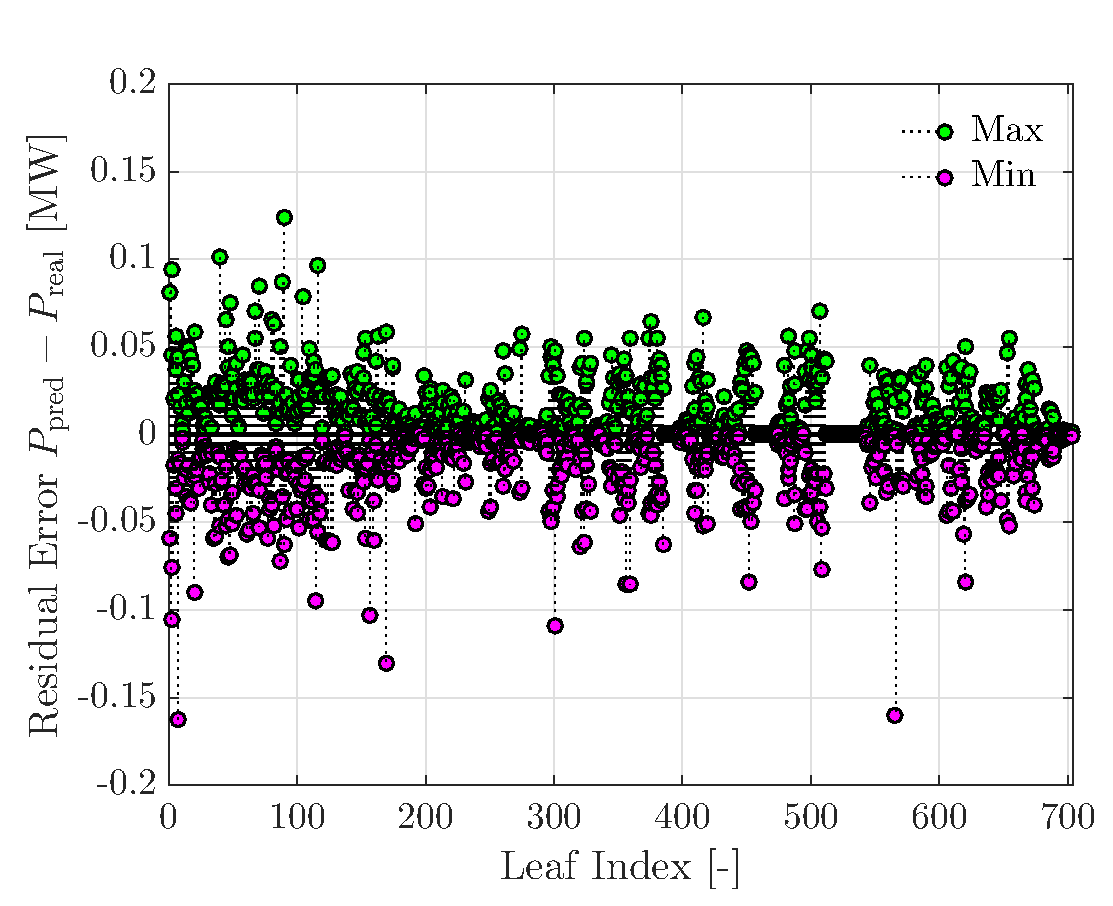
\includegraphics[width=20pc]{Figures/error_leaf.eps}
%\caption{The tree has 703 leaves. For each leaf, a maximum and a minimum error in prediction of average power consumption over the control horizon $\mathcal{P}_{\mathrm{pred}}-\mathcal{P}_{\mathrm{act}}$ is calculated from the data points that end up in that leaf. }
%\captionsetup{justification=centering}
%\label{F:linear_approx}
%\end{figure}
For 2 randomly selected leaves, the fit of the linear model against the actual power consumption is shown in Fig. \ref{F:linear_approx2}. The error observed in the predicted and actual power consumption for all leaves is depicted in Fig. \ref{F:linear_approx}.
It can be seen that for a small number of samples in the leaves of the tree the linear model assumption is valid.

